\chapter{Alternative Implementierungen der Bibliotheken und Frameworks des BDAS}
\label{chapter:alternative implementierungen}








Wie in den Abbildungen \ref{fig:BDAS1} und \ref{fig:bdas]} im vorhergehenden Kapitel ersichtlich ist, existieren auf jeder Ebene des BDAS auch alternative Implementierungen. Im folgenden Kapiteln werden einige Alternativimplementierungen vorgestellt und den Bibliotheken aus dem BDAS gegenübergestellt. Hier wird gezeigt, dass Spark Streaming, je nach Nutzungskontext durch Apache Storm ersetzt werden, oder statt der mitgelieferten Machine Learning Library MLLibs H2O oder Dato GraphLab Create\textsuperscript{TM} eingesetzt werden kann.  


\section{Alternative zu Spark: Apache Flink}
\label{section:apache flink}

Bei Apache Flink handelt es sich um ein weiteres verteiltes Big Data Analytics Framework. Somit stellt es eine mögliche Alternativimplementierung für Apache Spark dar. Flink ist aus einem Forschungsprojekt der Technischen Universität Berlin, der Humboldt Universität Berlin und des Hasso Plattner Instituts hervorgegangen. Hier wurde unter dem Projektnamen Stratosphere laut \citelit{stra13} ein System zur massiven Parallelverarbeitung von großen strukturierten und unstrukturierten Datenmengen entwickelt. 2014 wurde es zu einem Apache Incubating Project und im Zuge dessen in Apache Flink umbenannt. 

Erklärtes Ziel von Flink ist ein möglichst einfach zu programmierendes und für Entwickler transparentes Big Data Analytics Framework. Dies wird durch intuitive Abstraktionen von datenintensiven Berechnungsmodellen innerhalb der APIs umgesetzt. Derzeit existieren APIs für die Programmiersprachen Java und Scala, weitere sind in Planung. 

Eine Besonderheit von Flink ist die Übersetzung von \textit{High-Level-Operatoren} wie \textit{map, reduce, filter, join, intersect,} etc.  in \textit{Dataflow DAGs}\footnote{Ein DAG ist ein Directed Acyclic Graph. Im Kontext der Parallelverarbeitung in verteilten Systemen repräsentiert dieser die Pfade durch den Kontrollflussgraphen, der benötigt wird, um den Datenfluss zu berechnen.} (Vergleich \citelit{dag02}). Diese Übersetzung beinhaltet Optimierungsfunktionen, die auf den jeweiligen Datenflusskosten basieren. Wenn die zugrundeliegenden Daten oder die Clusterkonfiguration sich ändern, ist eine Anpassung der Flink-Anwendungen so mit sehr wenig Aufwand verbunden. 

Flink nutzt, ähnlich wie Spark, ebenfalls eine aggressive In-Memory-Strategie für seine Berechnungen. Wenn der zur Verfügung stehende Hauptspeicher für die benötigten Daten nicht ausreicht, werden interne Operationen auf die im Festspeicher persistierten Daten ausgelagert und ermöglichen so laut \citeint{flc14} eine sehr robuste Ausführung auf Systemen jeglicher Hauptspeicherausstattung. 

Ebenfalls vergleichbar mit Spark ist die Ausstattung mit Bibliotheken für Anwendungen wie Streaming, Graphen-Anwendungen, Machine Learning und SQL-Abfragen. 

Auch im Handling und im Umgang mit den Datenstrukturen existieren einige Gemeinsamkeiten zwischen Apache Flink und Apache Spark. In beiden Frameworks wird bei der Verarbeitung der Daten mittels \textit{Lazy Evaluation} vorgegangen (Vergleich Kapitel \ref{section:rdd}). Im Falle von Spark wird das Laden und Transformieren der Daten bei Aufruf einer \textit{Function} ausgeführt, bei Flink entspricht dies den \textit{Execute Methods}. Auch die Transformationen sind sehr ähnlich gegenüber Spark umgesetzt. In der Tabelle \ref{tab: flink transformations} (Inhalt aus \citeint{fpg15}, hier ist die vollständige Übersicht über alle Transformationen zu finden) sind einige Transformationen exemplarisch aufgeführt. 


\begin{table}[!ht]
\centering
\begin{tabular}{| p{5cm} | p{8cm} | }
\hline
Transformation & Zweck \\ \hline \hline
map & Takes one element and produces one element.  \\ \hline 
filter & Evaluates a boolean function for each element and retains those for which the function returns true. \\ \hline 
flatMap & Takes one element and produces zero, one, or more elements.\\ \hline 
mapPartitions & Transforms a parallel partition in a single function call. The function get the partition as an Iterator and can produce an arbitrary number of result values. The number of elements in each partition depends on the degree-of-parallelism and previous operations. \\ \hline 
aggregate & Aggregates a group of values into a single value. Aggregation functions can be thought of as built-in reduce functions. Aggregate may be applied on a full data set, or on a grouped data set. \\ \hline 
union & Produces the union of two data sets. \\ \hline 

\end{tabular}
\caption{Übersicht der einiger wichtiger Transformationen von Apache Flink}
	\label{tab: flink transformations}
\end{table}


\begin{figure}[htb!]
\centering
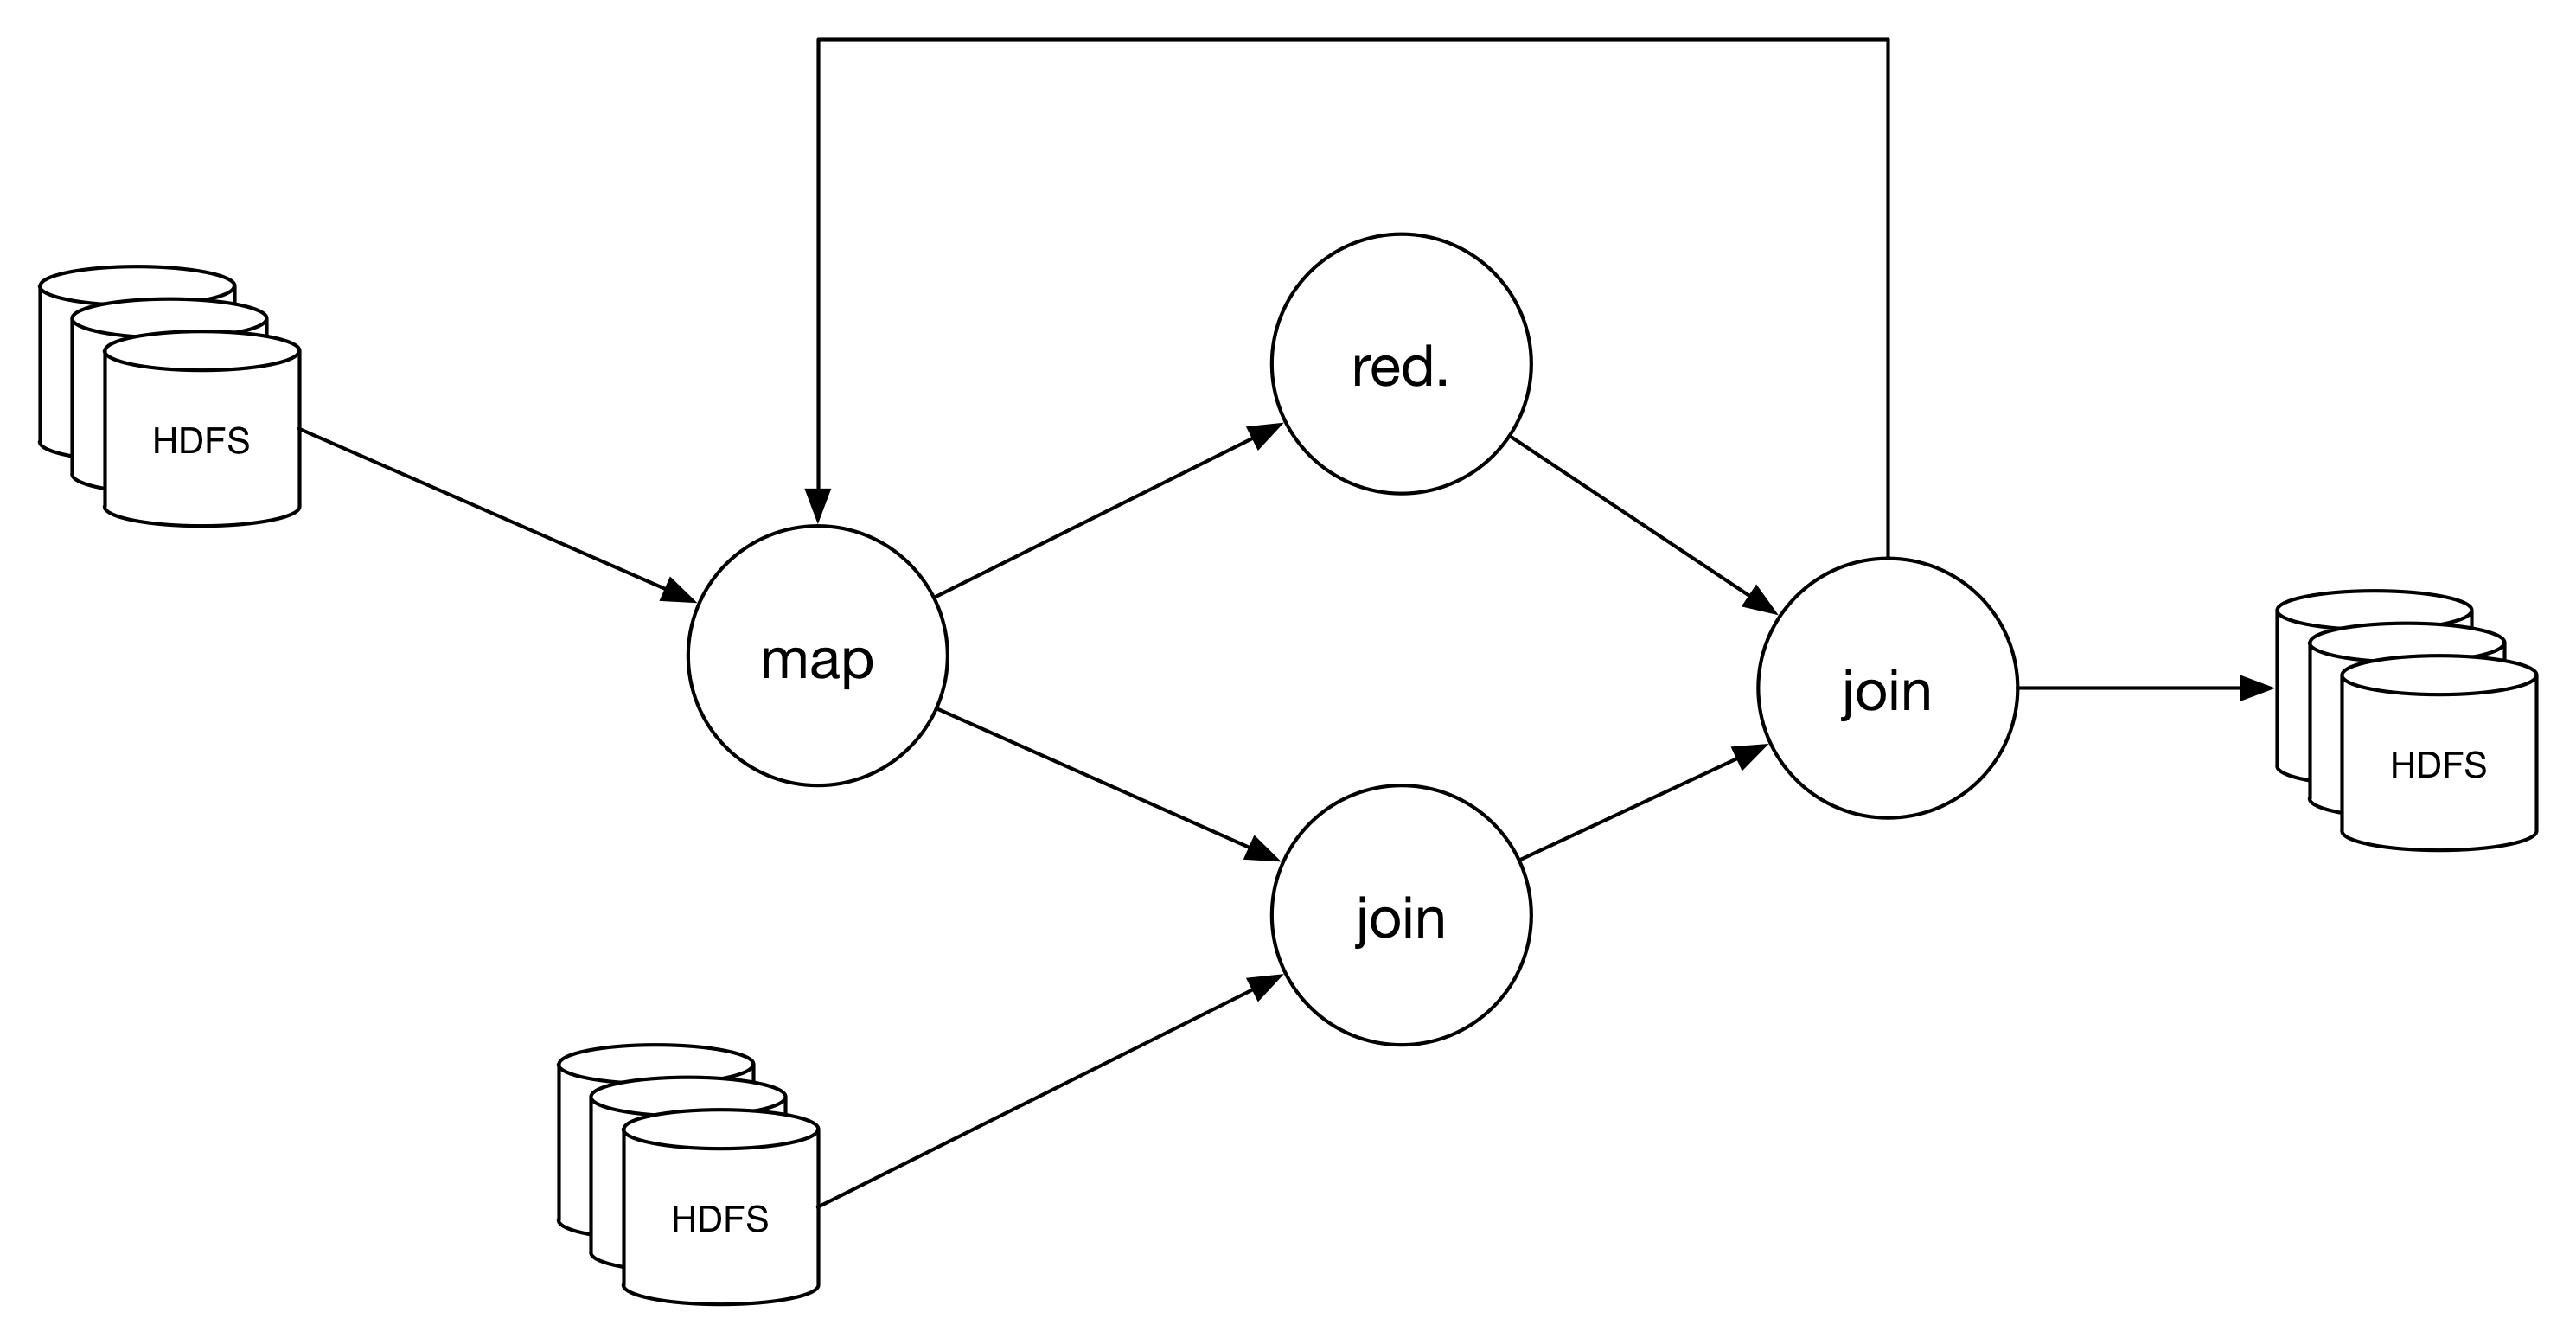
\includegraphics[width=1.0\textwidth]{bilder/flink.png}
\caption{Flink Streaming Dataflow mit Feedback führt bei Iterationen automatische Optimierungen durch.}
\label{fig:flink}
\end{figure} 

Unterschied zu Spark \citeint{afl14}



\section{Alternative zu Spark Streaming: Storm}
\label{section:storm}


Storm ist, wie Apache Streaming, ein Framework für Hadoop, bzw. Spark für verteilte Streaming-Anwendungen. Wo Spark ganz klar eine Verbesserung gegenüber Hadoop darstellt und Spark SQL dementsprechend gegenüber Hive, ist die Situation bei Storm und Apache Streaming hingegen nicht so klar determinierbar. 

Storm und Spark Streaming unterscheiden sich fundamental in ihren Verarbeitungsmodellen \citeint{va14}. Das erstgenannte Framework verarbeitet eintreffende Events nacheinander, immer genau eines pro Zeitraum. Spark Streaming sammelt im Gegensatz dazu die Events in Mini-Batch-Jobs und verarbeitet sie paketweise zu definierten Zeiträumen nach wenigen Sekunden. Deshalb kann Storm Latenzzeiten von deutlich unter einer Sekunde erreichen, während Spark Streaming eine Latenzzeit von einigen Sekunden aufweist. Diesen Nachteil macht Spark Streaming durch eine sehr gute Fehlertoleranz wett, da die Mini-Batches nach aufgetretenen Fehlern einfach nochmals bearbeitet werden können und die zuvor fehlerhaft ausgeführte Verarbeitung verworfen wird. Treten hingegen bei Storm Fehler auf, wird genau dieser Datensatz nochmals verarbeitet. Dies bedeutet, dass dieser auch mehrfach verarbeitet werden kann. Durch dieses Verhalten lassen sich die beiden Frameworks grob in zwei Einsatzgebiete verteilen:

Storm ist das Framework der Wahl, wenn Wert auf sehr kurze Latenzzeiten gelegt werden muss, hingegen ist es für statusbehaftete Anwendungen durch die Möglichkeit der Mehrfachverarbeitung ungeeignet. Im Umkehrschluss ist Spark Streaming eine gute Wahl, wenn aufgrund der gestreamten Daten eine Statusmaschine aufgebaut werden soll. Dafür müssen hier höhere Latenzzeiten in Kauf genommen werden.     

\section{Alternative zu MLLibs: H2O - Sparkling Water}
\label{section:h20}


BluBlaBlubb


\section{Alternative zu MLLibs: Dato GraphLab Create\textsuperscript{TM}}
\label{section:h20}


BluBlaBlubb



\subsection{Zusammenfassung}
\label{section:storm}




